\documentclass[10pt,a4paper]{article}
\usepackage[utf8]{inputenc}
\usepackage[spanish]{babel}
\usepackage{amsmath}
\usepackage{amsfonts}
\usepackage{amssymb}
\usepackage{enumitem}
\usepackage{hyperref} 
\usepackage{graphicx}
\usepackage[table]{xcolor}
\hypersetup{pdftex,colorlinks=true,allcolors=black}

\hypersetup{
    pdftitle={},
    pdfauthor={Pablo Riutort Grande},
    pdfsubject={},
    bookmarksnumbered=true,     
    bookmarksopen=true,         
    bookmarksopenlevel=1,       
    colorlinks=true,            
    pdfstartview=Fit,           
    pdfpagemode=UseOutlines,    % this is the option you were lookin for
    pdfpagelayout=TwoPageRight
}
\usepackage{listings}
\usepackage{xcolor}
\usepackage{hypcap}
\definecolor{codegreen}{rgb}{0,0.6,0}
\definecolor{codegray}{rgb}{0.5,0.5,0.5}
\definecolor{codepurple}{rgb}{0.58,0,0.82}
\definecolor{backcolour}{rgb}{0.95,0.95,0.92}
\lstdefinestyle{mystyle}{
    backgroundcolor=\color{backcolour},   
    commentstyle=\color{codegreen},
    keywordstyle=\color{magenta},
    numberstyle=\tiny\color{codegray},
    stringstyle=\color{codepurple},
    basicstyle=\ttfamily\footnotesize,
    breakatwhitespace=false,         
    breaklines=true,                 
    captionpos=b,                    
    keepspaces=true,                 
    numbers=left,                    
    numbersep=5pt,                  
    showspaces=false,                
    showstringspaces=false,
    showtabs=false,                  
    tabsize=2
}

\lstset{style=mystyle}
\usepackage{xparse}
\NewDocumentCommand{\codeword}{v}{%
\texttt{{#1}}
}
\author{Pablo Riutort Grande}
\title{
	Seguridad del software\\
	\vspace{0.5cm}
	PEC 1\\
	\vspace{1cm}
	\textbf{Debugging y reversing de una aplicación}
	\vspace{1cm}\\UOC - MISTIC
}


% ¿Qué habéis deducido o que hace la aplicación a partir del reversing realizado? ¿Cómo habéis llegado a esta conclusión?
% ¿Usa constantes, literales? ¿Cuáles son y qué uso tienen en la aplicación?
% ¿Qué bucles hay en la aplicación? ¿Qué hacen? ¿Cuáles son de tipo For, While o Do While? ¿Cómo o qué condicionante hay para salir del bucle? ¿Hay algun bucle anidado?
% ¿Qué métodos o funciones tiene la aplicación?
% ¿Habéis detectado algún punto vulnerable?
% ¿Utiliza alguna función vulnerable como por ejemplo strcpy, strcmp, a alguna otra?
% ¿Qué condicionales has encontrado? ¿Qué condición realiza? ¿Qué hace en cada caso?
% ¿Puedes detectar qué variables utiliza?
% Muestra el uso de la Pila en algún punto de la ejecución
% ¿Se puede alterar el flujo del código?


\begin{document}
\maketitle

\pagebreak
\tableofcontents
\listoffigures

\pagebreak

\section{Introducción}
Para este ejercicio se ha instalado y utilizado la herramienta de análisis de binarios e ingeniería inversa radare2 \cite{radare}. El binario analizado ha sido proporcionado por crackmes.one que es un servicio que proporciona binarios para analizar \cite{crackmes}, se ha seleccionado un binario de nivel 1 compilado en C para sistemas operativos Unix/Linux \cite{guess}.\\
En la sección de reversing se analiza el binario mencionado ... [completar una vez terminado el ejercicio].\\

El reverse engineering es un proceso complicado así que Radare es un software basado en interfaz de línea de comandos donde se puede especificar en cada momento qué se desea hacer sobre el binario. Para interactuar con él hay que introducir distintos comandos con distintos parámetros [Fig. \ref{fig:r2commands}].\\

\begin{figure}[h!]
  \centering
  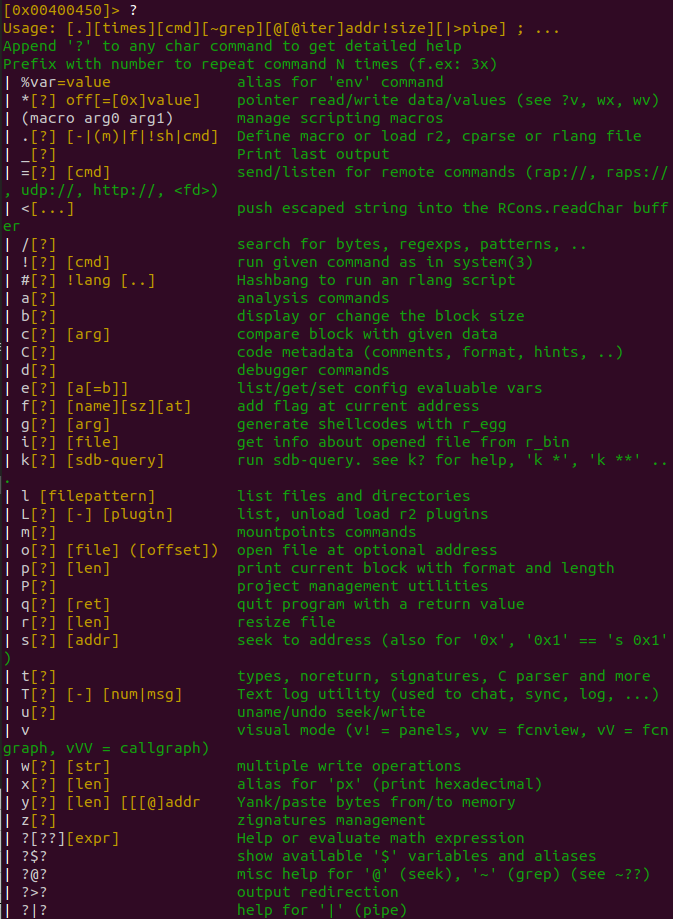
\includegraphics[scale=0.4]{r2commands.png}\\
  \caption{Comandos de r2}
  \label{fig:r2commands}
\end{figure}

\pagebreak

\section{Reversing}
El reversing se ha realizado con radare2 sobre el binario llamado ``guess\_my\_name'', el primer paso es importar el binario con radare y hacer un análisis del mismo.\\
\begin{figure}[h!]
  \centering
  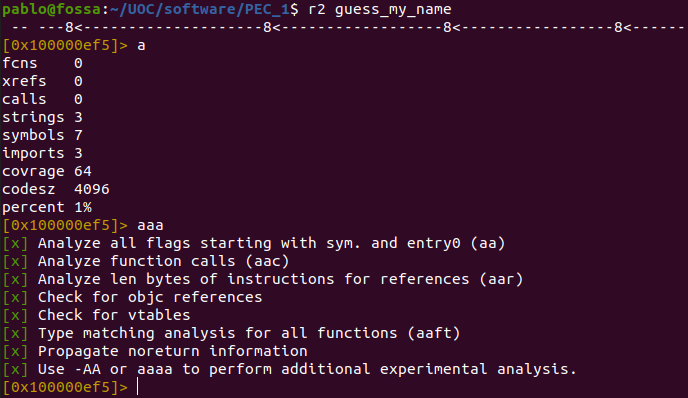
\includegraphics[scale=0.5]{r21.png}\\
  \caption{Análisis del binario}
  \label{fig:r21}
\end{figure}

El comando 'a' realiza un análisis del binario. Existen varios niveles de análisis con radare, se ha utilizado el más exhaustivo [Fig. \ref{fig:aa}]. También existen distintas variantes de 'a', más adelante se utilizará para listar funciones y variables \cite{radare}.

\begin{figure}[h!]
  \centering
  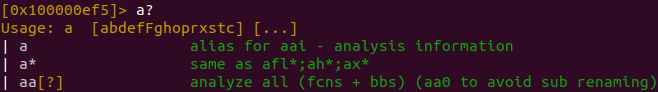
\includegraphics[scale=0.4]{aa.png}\\
  \caption{Comando 'a'}
  \label{fig:aa}
\end{figure}

Después de este análisis ya tendremos suficiente información como para consultar los flags del binario. Los flags nos aportan información muy interesante ya que asocian un nombre con un offset del archivo y además se agrupan en namespaces, algunos de estos namespaces (flag spaces) son secciones, funciones, símbolos y strings [Fig. \ref{fig:flags}] \cite{radarebook}.

\begin{figure}[h!]
  \centering
  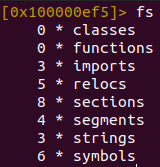
\includegraphics[scale=0.7]{fs.png}\\
  \caption{Flags del binario}
  \label{fig:flags}
\end{figure}

Para listar strings podemos seleccionar el flag space de strings \ref{fig:strings}. Vemos que se listan 3 strings: ``What's my name'', ``mrmtg'' y ``You got it''.
\begin{figure}[h!]
  \centering
  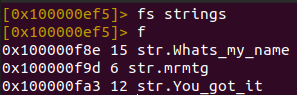
\includegraphics[scale=0.7]{strings.png}\\
  \caption{Listado de strings del binario}
  \label{fig:strings}
\end{figure}

Si listamos las funciones veremos que radare encuentra 4, 3 de sistema y 1 propia llamada ``entry0''. Las funciones de sistema son ``puts'', ``gets'' y ``strcmp'', estas funciones son vulnerables al buffer overflow que ocurre cuando los datos se escriben sobrepasando los límites de memoria reservada para una estructura de datos en particlar. En C se definen los strings como un array de caracteres terminados por el carácter ``null'' y no se realiza una comprobación de límites de estos arrays incluso en las librerías estándard del lenguaje; si el tamaño del string es demasiado grande se produce el desbordamiento y puede provocar un comportamiento no deseado del programa \cite{buffer_overflow}.\\

Para ver el contenido de la pila en Radare podemos utilzar el comando ``px'' que se utiliza para mostrar el contenido en hexadecimal de la memoria, en este caso, para apuntar al contenido de la pila podemos usar ``rsp'': ``pxa @ rsp'' \cite{rsp} [Fig. \ref{fig:stack}].

\begin{figure}[h!]
  \centering
  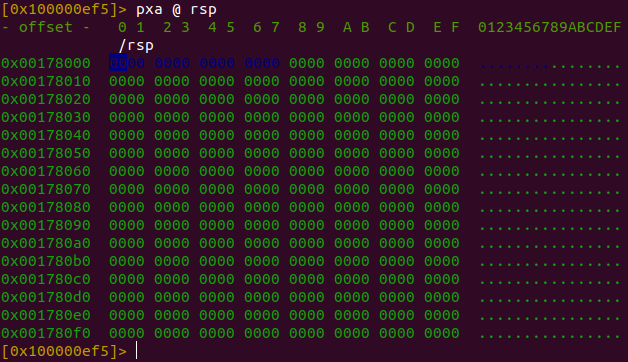
\includegraphics[scale=0.5]{pxa.png}\\
  \caption{Comando para ver el contenido de la pila en Radare}
  \label{fig:stack}
\end{figure}

\section{Análisis de la función principal}
La función ``entry0'' hace la función de main tal y como podemos ver en la dirección de memoria 0x100000ef5 que coincide con el nombre de ``main''.

\begin{figure}[h!]
  \centering
  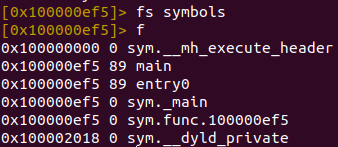
\includegraphics[scale=0.5]{main_entry0.png}\\
  \caption{entry0 tiene la misma dirección de memoria que main}
  \label{fig:pdf}
\end{figure}

Para ver el cuerpo de la función podemos utilizar el comando seek sobre el nombre de la función para buscar el la función ``entry0'': 's entry0'. Posteriormente podemos ejecutar el comando ``pdf'' para ver la función seleccionada desensamblada. Tanto en el cuerpo de la función como con el comando ``afv'' podemos ver la declaración de variables, en nuestro binario encontramos ``char *s1'' \cite{radarebook} [Fig. \ref{fig:pdf}].\\

Si analizamos detenidamente la función desensamblada podemos ver que primero se muestra por pantalla el string ``What's my name'' [Fig. \ref{fig:pdf1}], seguido de la función fgets que lee una línea de un stream especificado y lo guarda en una variable [Fig. \ref{fig:pdf2}]. Esta variable es luego comparada con otro string asignado a ``mrmtg'' mediante la función strcmp [Fig. \ref{fig:pdf3}]. Si el resultado de esta comparación no es positivo, entonces saltamos a la dirección de memoria 0x100800f09, en caso contrario se muestra el string ``You got it!'' [Fig. \ref{fig:pdf4}].\\

De este comportamiento, podemos deducir que el programa hace una comparación con el string ``mrmtg'', en caso de no coincidir saltamos a otra dirección de memoria en bucle.

\begin{figure}[h!]
  \centering
  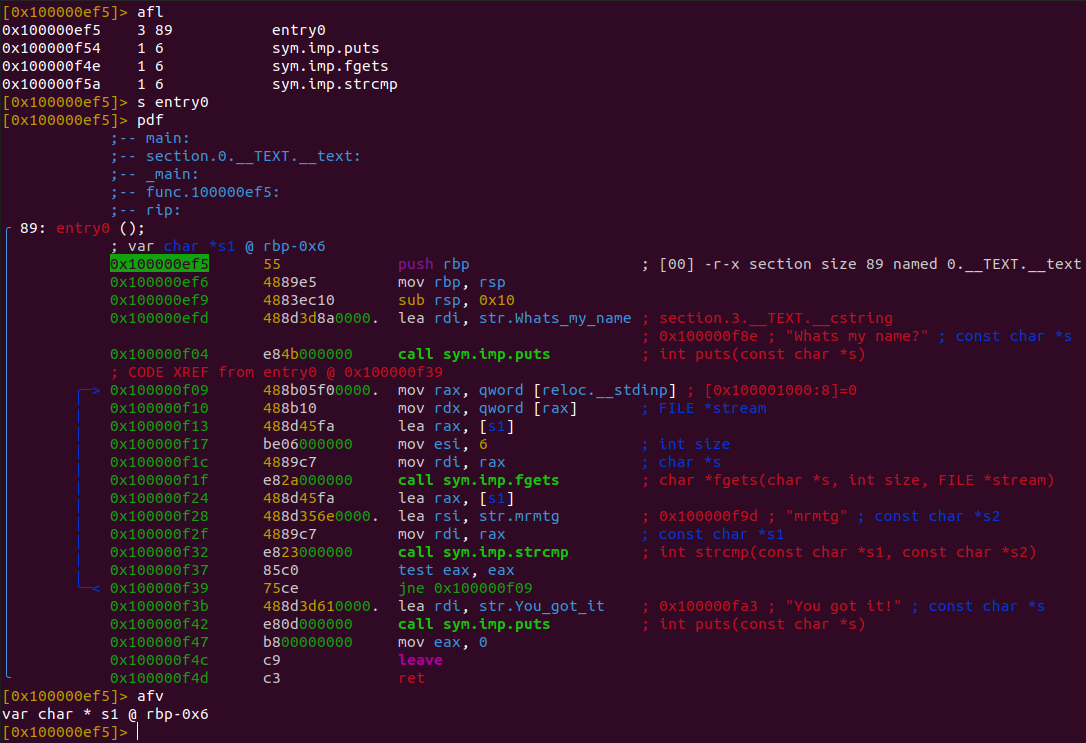
\includegraphics[scale=0.3]{pdf.png}\\
  \caption{Print Disassembled Function}
  \label{fig:pdf}
\end{figure}

\begin{figure}[h!]
  \centering
  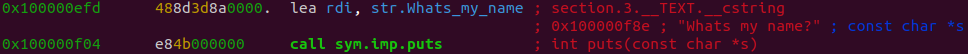
\includegraphics[scale=0.3]{puts.png}\\
  \caption{PDF: Sección de la primera función puts}
  \label{fig:pdf1}
\end{figure}

\begin{figure}[h!]
  \centering
  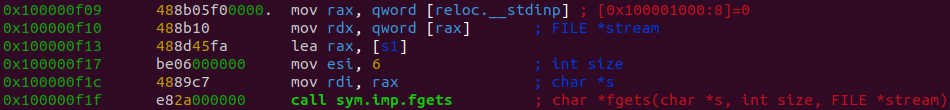
\includegraphics[scale=0.3]{fgets.png}\\
  \caption{PDF: Sección de la función fgets}
  \label{fig:pdf2}
\end{figure}

\begin{figure}[h!]
  \centering
  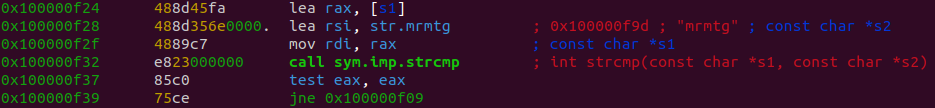
\includegraphics[scale=0.3]{strcmp.png}\\
  \caption{PDF: Sección de la función strcmp}
  \label{fig:pdf3}
\end{figure}

\begin{figure}[h!]
  \centering
  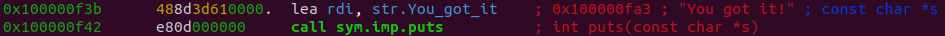
\includegraphics[scale=0.3]{puts2.png}\\
  \caption{PDF: Sección de la segunda función puts}
  \label{fig:pdf4}
\end{figure}

A continuación tenemos una aproximación de lo que podría ser el código fuente del programa, un bucle continuo mediante ``do while'' que recibe el input estándard y lo compara con el string "mrmtg", en caso de acierto muestra el string ``You got it!'' y finaliza el programa.
\lstinputlisting[language=C]{gmn.c}

\pagebreak

\subsection{Vista gráfica}
En radare existe el modo gráfico que nos permite ver el flujo del binario, podemos acceder a este modo mediante el comando ``VV'' [Fig. \ref{fig:vv}].\\

\begin{figure}[h!]
  \centering
  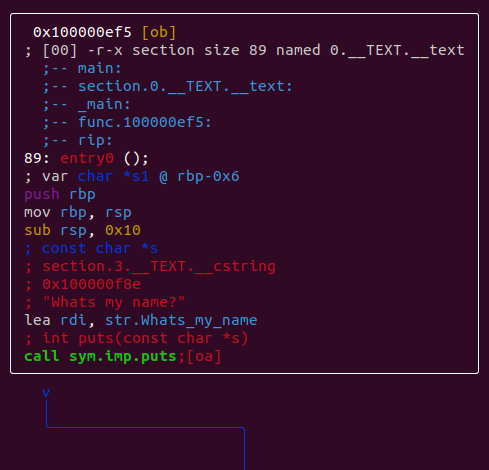
\includegraphics[scale=0.35]{vb1.png}\\
  \caption{Primer bloque del modo gráfico}
  \vspace{0.3cm}
  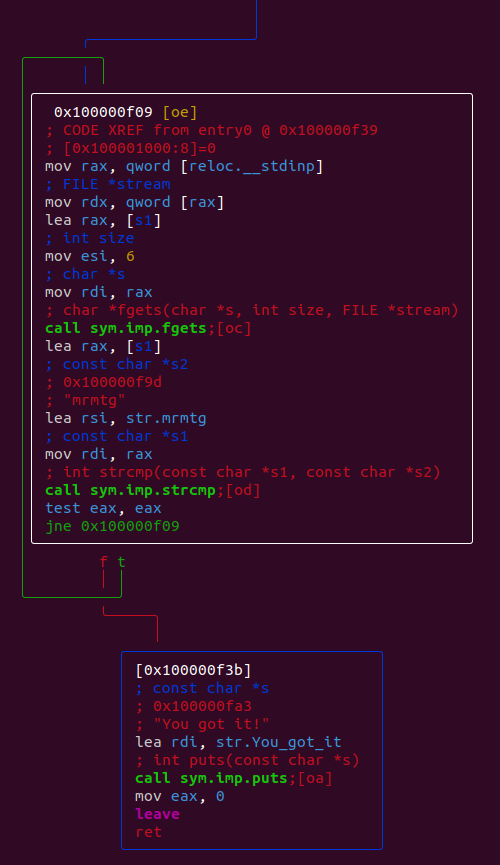
\includegraphics[scale=0.35]{vb2.png}\\
  \caption{Segundo bloque del modo gráfico}
  \label{fig:vv}
\end{figure}

\pagebreak

En este modo también se puede ver con más detalle las variables declaradas y otras constantes que se utilizan en las funciones llamadas en el binario [Fig. \ref{fig:variables}].

\pagebreak
\begin{lstlisting}[language=C]
const char *s;
int puts(const char *s);
\end{lstlisting}

\begin{lstlisting}[language=C]
FILE *stream;
int size = 6;
char *s;
char *fgets(char *s, int size, FILE *stream);
\end{lstlisting}

\begin{lstlisting}[language=C]
const char *s2;
const char *s1;
int strcmp(const char *s1, const char *s2);
\end{lstlisting}

\begin{lstlisting}[language=C]
const char *s;
int puts(const char *s)
\end{lstlisting}

En la asignación de strings a variables se ejecuta el mnemónico ``lea rdi, str.$<$String$>$'' donde ``lea'' es el opcode de \textit{Load Effective Address} que carga la dirección efectiva del string en el registro \textit{rdi}, usado como puntero destino.\\
En la declaración de arrays de tipo char está el mnemónico ``mov rdi, rax''. El registro \textit{rdi} contiene la dirección de memoria del array y la instrucción copia el contenido del registro \textit{rax} (Registro acumulador o de propósito general) al primer elemento del array.\\
La declaración de la variable de tipo entero ``size'' consiste en mover el valor 6 al registro \textit{esi}, que es un registro utilizado como puntero.

\begin{figure}[h!]
  \centering
  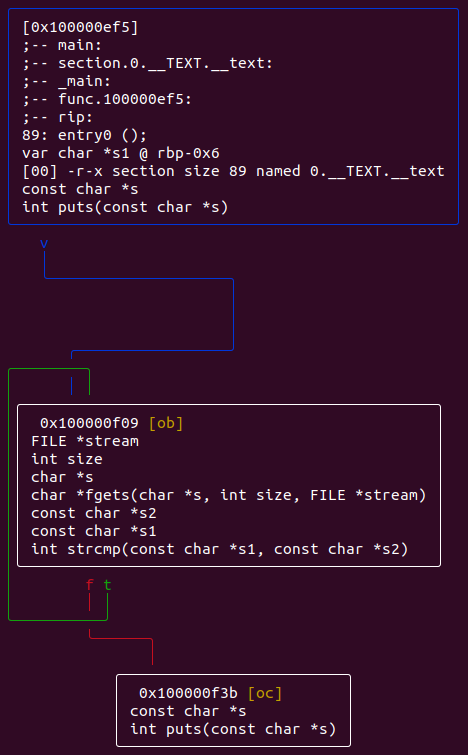
\includegraphics[scale=0.35]{variables.png}\\
  \caption{Variables de las funciones}
  \label{fig:variables}
\end{figure}

\section{Alterar el flujo del código}
Como ya se ha comentado anteriormente, las funciones ``puts'', ``gets'' y ``strcmp'' son vulnerables al buffer overflow y estas pueden ser atacadas si la entrada se prepara de forma especial para corromper la ejecución del stack del programa. En el siguiente ejemplo  el código utiliza la función vulnerable gets() para leer datos en un buffer. Como no hay limitación de tamaño para la lectura de estos datos en la función depende del usuario el introducir los datos del tamaño adecuado al buffer \cite{buffer_overflow2}.

\begin{lstlisting}[language=C]
...
char buf[BUFSIZE];
gets(buf);
...
\end{lstlisting}

Si accede a la pila de ejecución con la técnica de buffer overwlor se podrían introducir instrucciones de alto nivel como sacar una shell.

\subsection{Patching}
Otra alternativa para cambiar el comportamiento del binario es cambiando el binario en sí. Para eso se puede ver el código decompilado y decidir qué bytes se tienen que cambiar para modificar el comportamiento como, por ejemplo, cambiando alguna condición de salto \cite{patching}.\\
En Linux tenemos el comando ``xxd'' que crea un dump en hexadecimal de un archivo o del input estándar, podemos ver el contenido de un binario con este comando [Fig. \ref{fig:hex}].

\begin{figure}[h!]
  \centering
  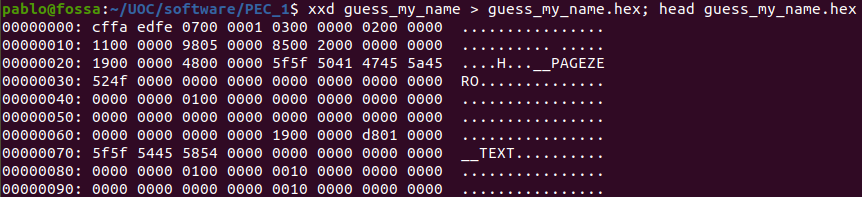
\includegraphics[scale=0.4]{hex.png}\\
  \caption{Hexadecimal del binario guess\_my\_name}
  \label{fig:hex}
\end{figure}

En nuestro binario tenemos una única condición de salto (jne) y es la candidata idónea para ser modificada de tal forma que cambie el flujo del programa. Esta condición de salto se encuentra en la dirección 0x000011cd la cual podemos encontrar en el hexadecimal para buscar mejor nuestra instrucción de salto.\\

El opcode del mnemónico según la documentación del procesador empieza por 75c, si buscamos ese número en el dump en hexadecimal lo podremos modificar por 74c0 que es el opcode del mnemónico JE (Jump short if equal) \cite{opcode}. Una vez modificado podemos restaurar un binario nuevo a partir del nuevo hexadecimal y ejecutarlo para ver que el comportamiento se ha modificado [Fig. \ref{fig:hex}].

\begin{figure}[h!]
  \centering
  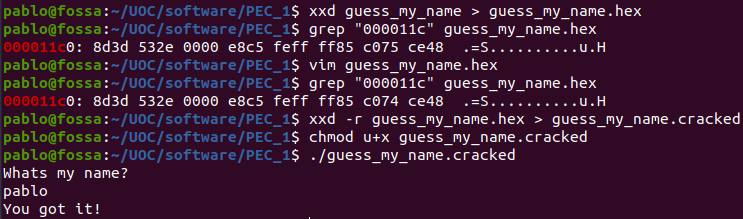
\includegraphics[scale=0.5]{cracked.png}\\
  \caption{Cambio del código hexadecimal del binario}
  \label{fig:hex}
\end{figure}

\pagebreak

\begin{thebibliography}{9}

\bibitem{radare}
	\textbf{radare2}\\
	Radare2 is a complete framework for reverse-engineering and analyzing binaries\\
	\url{https://rada.re/n/radare2.html}

\bibitem{crackmes}
	\textbf{crackmes.one}\\
	This is a simple place where you can download crackmes to improve your reverse engineering skills.\\
	\url{https://crackmes.one/}

\bibitem{guess}
	\textbf{crackmes.one}\\
	mrmtg's Guess\_my\_name\\
	\url{https://crackmes.one/crackme/5ed0584b33c5d449d91ae67b}
	
\bibitem{radarebook}
	\textbf{Radare2 Book}\\
	Flags \url{https://radare.gitbooks.io/radare2book/content/basic_commands/flags.html}\\
	Code Analysis \url{https://radare.gitbooks.io/radare2book/content/analysis/code_analysis.html}\\
	Hexadecimal View \url{https://radare.gitbooks.io/radare2book/content/basic_commands/print_modes.html}\\
	Variables \url{https://radare.gitbooks.io/radare2book/content/analysis/variables.html}\\
	Vidual Mode \url{https://radare.gitbooks.io/radare2book/content/visual_mode/intro.html}\\
	
\bibitem{buffer_overflow}
	\textbf{Secure Coding in C and C++: Strings and Buffer Overflows}\\
	Robert C. Seacord, Apr 24, 2013\\
	\url{https://www.informit.com/articles/article.aspx?p=2036582&seqNum=3}
	
\bibitem{buffer_overflow2}
	\textbf{OWASP}\\
	Buffer Overflow\\
	\url{https://owasp.org/www-community/vulnerabilities/Buffer_Overflow}

\bibitem{rsp}
	\textbf{Stack Exchange - Reverse Engineering}\\
	How to get a nice stack view in radare2?\\
	\url{https://reverseengineering.stackexchange.com/questions/16844/how-to-get-a-nice-stack-view-in-radare2}
	
\bibitem{patching}
	\textbf{Using Radare2 to patch a binary}\\
	Derik Ramirez, Dec 28 2019.\\
	\url{https://rderik.com/blog/using-radare2-to-patch-a-binary/}

\bibitem{opcode}
	\textbf{Intel Pentium Instruction Set Reference (Basic Architecture Overview)}\\
	JNE - Jump if Condition Is Met\\
	\url{http://faydoc.tripod.com/cpu/jne.htm}

\end{thebibliography}

\end{document}